%!TEX root = main.tex

\subsection{The problem}

Align three or more homologuous sequences (globally or localy).

\subsubsection{Scoring}

\begin{figure}[H]
	\centering
	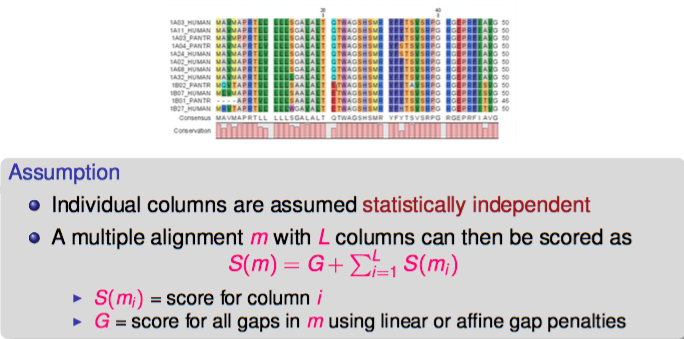
\includegraphics[scale=0.6]{images/32_assumptions.png}
	\caption{Assumptions.}
\end{figure}

\begin{figure}[H]
	\centering
	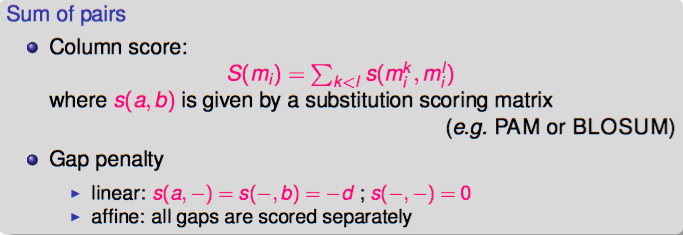
\includegraphics[scale=0.6]{images/33_sums.png}
	\caption{Sum of pairs.}
\end{figure}

\subsection{Dynamic programming}

Optimal alignment between k sequences can be computed with DP. With an average length of $\bar{n}$, the time complexity is $O(2^k \bar{n}^k)$ and the space complexity is $O(\bar{n}^k)$ (hyper cube).

One algorithm which compute optimally the alignement is \textbf{MSA} algorithm ($O(k^2 \bar{n}^2)$: 10 sequences of 200-300 residues in reasonnable time).
\begin{figure}[htp]
	\centering
	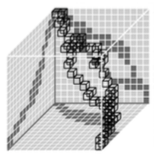
\includegraphics[scale=0.5]{images/34_msa.png}
	\caption{MSA.}
\end{figure}

\begin{itemize}
	\item Compute all pairwise alignments;
	\item Limits the exploration of the hyper cube to regions consitent with those alignments.
\end{itemize}

\textbf{G-MSA} is an optimization: 500 sequences of 236 residues in 10 seconds.

\subsubsection{Progressive alignment methods (greedy heuritic)}

\begin{figure}[htp]
	\centering
	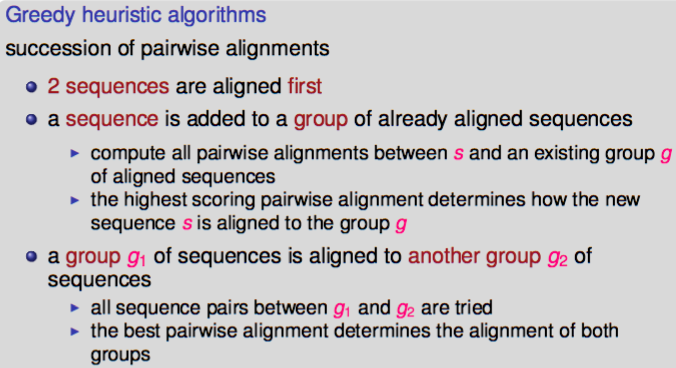
\includegraphics[scale=0.5]{images/35_greedy.png}
	\caption{Greedy heuritic.}
\end{figure}

There are some limitations:
\begin{itemize}
	\item the degree of sequence conservation at each position should be taken into account;
	\item mismatches at highly conserved positions should be more penalized;
	\item the order in which sequences are incorporated in the multiple alignment matters.
\end{itemize}
\newpage
\paragraph{ClustalW}

\begin{center}
	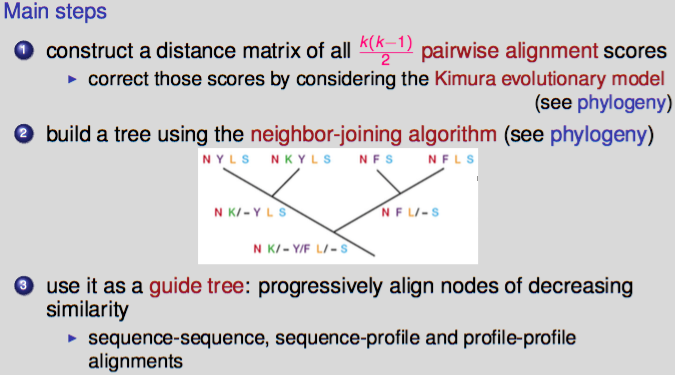
\includegraphics[scale=0.5]{images/36_clustalW.png}
\end{center}

There can be further heuristics:
\begin{itemize}
	\item \textbf{position specific gap open penalties with decreased penalties} wherever other gaps have been found amoung already aligned sequences;
	\item gap penalties are also decreased or increased based on a large collection of \textbf{structural alignments};
	\item the guide tree may be ajusted \textbf{on the fly} to defer a low scoring alignment until more profile information has been accumulated.
\end{itemize}

